  \section{View}

  \subsection{Implementation}

  The \textbf{View} is responsible for rendering \textbf{Model} onto the GUI and the hardware peropherals.
  It possessed routines that the \textbf{Model} uses to trigger updates to the GUI and peripherals.
  This implementation was chosen as updates can be triggered as and when the \textbf{Model} is updates and in a time-triggered fashion..

  The GUI component of the \textbf{View} holds many strings with ANSI escape sequences.
  Some of these stored strings are used to do the following:

  \begin{itemize}
    \item Change location of cursor (see \textbf{Listing \ref{lst:esc-cursor-pos}}).
    \item Display game stats (time left, current refresh interval, level, high score, current score, etc).
    \item Print empty board (just walls).
  \end{itemize}

    \begin{lstlisting}[caption={Escape sequence to change cursor position},label={lst:esc-cursor-pos}]
ESC_cursor_position	= 27,"["    ; Beginning of escape sequence
ESC_cursor_pos_line	= "000"     ; This can be changed in code to change row
ESC_cursor_pos_sep	= ";"
ESC_cursor_pos_col	= "000"     ; This can be changed in code to change column
ESC_cursor_pos_cmd	= "f",0     ; End of sequence

  \end{lstlisting}


  \subsection{GUI Operations (\textit{PuTTY} output)}

%  \begin{table}[H]
%  \begin{tabular}{rl}
%    \texttt{FILE}:         &\texttt{gui.s}  \\
%    \texttt{PRIMARY CONTRIBUTOR}:    &\texttt{Anand Balakrishnan (anandbal)}
%  \end{tabular}
%  \end{table}

   The \textbf{View} also holds routines whose primary function is to use these strings and manipulate GUI.
    It exposes the following subroutines so as to allow the \textbf{Model} to trigger updates to GUI.

    \begin{itemize}
      \item \texttt{draw\_empty\_board}
      \item \texttt{populate\_board}
      \item \texttt{update\_board}
      \item \texttt{clear\_sprite}
    \end{itemize}


 
    \subsubsection{Board Initialization}

    The subroutines \texttt{draw\_empty\_board} and \texttt{populate\_board} are responsible for displaying the game board before the game begins.
    The \texttt{draw\_empty\_board} subroutine does the following:

    \begin{enumerate}
      \item Output the string containing an empty board with the walls.
      \item Output the initial game stats, game legend and controls.
    \end{enumerate}

    The \texttt{populate\_board} subroutine does the following:

    \begin{enumerate}
      \item For each sprite in \textbf{Model}, read the X and Y positions, and display it on the board.
      \item For each coordinate on the board, check if the \textbf{Model} holds a block of sand at that coordinate and fill the board with sand accoding to the mode.
    \end{enumerate}

    \subsubsection{Update GUI}

    The subroutine responsible for updating the entire GUI is \texttt{update\_board}. It is also a relatively small routine and does the following:
    
    \begin{enumerate}
      \item Check if \texttt{GAME OVER}. If so, display Game Over GUI. Else.
      \item Erase all sprites by loading in their coordinates and printing a ` ' at each coordinate.
      \item For each sprite, check if the sprite is alive and print the appropriate GUI character at the sprite's current location.
      \item Display game stats.
    \end{enumerate}


  \subsection{Peripheral Operations/Updates}
 
  The subroutine \texttt{update\_peripherals}, updates the 7 segment display, the RGB LED,
  and monochrome LEDs. 
  This routine is triggered periodically by \textbf{Model} by through \texttt{update\_model}.
  This is responsible for displaying the game's states on the hardware
  peripherals. It reads the 4 game state variables, \texttt{RUNNING\_P}, \texttt{BEGIN\_GAME},
  \texttt{PAUSE\_GAME} and \texttt{GAME\_OVER}, and other variables like \texttt{LEVEL} and number of \texttt{LIVES}
  held by \textbf{Dug} to determine:
  
  \begin{enumerate}
    \item Color to display on the RGB LED.
    \item Number of LEDs to illuminate in the standard single-color LEDs.
    \item Number to display on the 7-segment display.
  \end{enumerate}

  \begin{figure}[H]
    \centering
    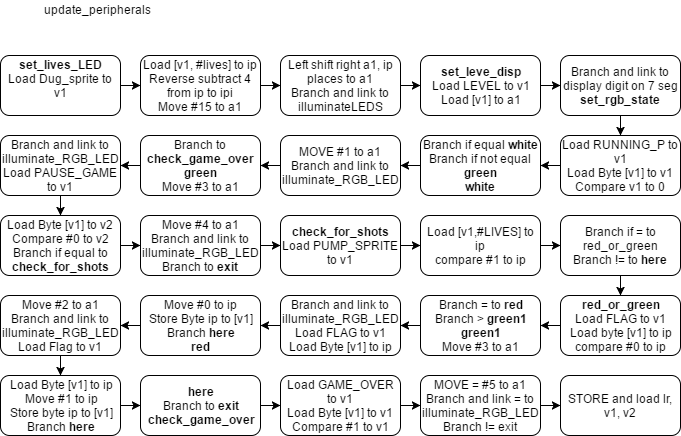
\includegraphics[width=0.75\textwidth]{images/update_peripherals.png}
  \end{figure}
